\documentclass[a4paper]{article}

%% Language and font encodings
\usepackage[spanish]{babel}
\usepackage[utf8x]{inputenc}
\usepackage[T1]{fontenc}

%% Sets page size and margins
\usepackage[a4paper,top=3cm,bottom=2cm,left=3cm,right=3cm,marginparwidth=1.75cm]{geometry}

%% Useful packages
\usepackage{amsmath}
\usepackage{graphicx}
\usepackage[colorinlistoftodos]{todonotes}
\usepackage[colorlinks=true, allcolors=blue]{hyperref}

\title{Algoritmos Genéticos - TIA}
\author{Carlos S. Galindo Jiménez}

\begin{document}
\maketitle
\section{Problema a resolver}
Ejemplo 5. Dado un conjunto de N bloques rectangulares, de distintas alturas y anchuras, se debe obtener la posición de todos los bloques en un espacio cartesiano bidimensional, tal que no haya solapamientos entre los bloques y se minimice la superficie  (anchura x altura)  del espacio contenedor. Asumid que los bloques no pueden girarse, es decir  siempre tienen una orientación determinada.

\section{Algoritmo genético}
\subsection{Diseño del individuo}
Cada individuo contiene un cromosoma, compuesto por $N$ genes, que contienen 2 números reales: la posición en el plano real de la esquina inferior derecha de cada bloque.

Si las dimensiones de los bloques están almacenadas en la matriz $M_{N\times D}$, cada pareja de coordenadas en cada gen $g$ tiene como valor mínimo $0$ y como valor máximo la suma del vector columna de $M$ apropiado (1 para $x$ y 2 para $y$).

La población inicial se puede generar con números aleatorios dentro del rango establecido.

\subsection{Función fitness}
La función fitness de este problema se puede definir como el la inversa del área cuadrada ocupada por los $N$ bloques en cada solución. En caso de que se den soluciones no factibles (si se produjera solapamiento), se puede generar otra solución factible desplazando vertical u horizontalmente los bloques en conflicto. Esto provoca un aumento del tamaño del espacio contenedor, por lo tanto disminuiría el fitness de la solución.

Se podría realizar la siguiente modificación a la función fitness: acercar lo más posible los bloques entre ellos antes de evaluar la función fitness antes mencionada, de tal modo que el cromosoma no represente la solución sino un ``despiece'' de los bloques. Esto tiene la ventaja que el fitness inicial puede ser mucho más alto, pero puede promover soluciones con máximos locales en el fitness, impidiendo que se llegue al máximo global. Por tanto si se implementa ese añadido, la probabilidad de mutación debe aumentar y el reemplazo debe ser lo suficiente rápido como para evitar el estancamiento.
\subsection{Generación de la nueva población}
\begin{itemize}
\item \textbf{Selección}: escogemos selección por rueda de ruleta, con una $p_i = \frac{f_i}{\sum_{j=1}^N f_j}$

\item \textbf{Cruce}: cualquier forma de cruce debe respetar el gen como unidad indivisible, puesto que una coordenada no tiene sentido sin la otra. Se podría seleccionar un cruce de 2 puntos (teniendo en cuenta que cada gen es un solo punto) o uno uniforme.

\item \textbf{Mutación}: la mutación por inserción no tiene sentido en este ejemplo, por lo que vamos a seleccionar mutación por intercambio recíproco, con una probabilidad $p_{mut}=0.01$. Además conviene dar otra pequeña probabilidad ($p_{mut2}=0.02$) a otro tipo de mutación, que consistiría en mover el un bloque una cantidad dada en una de las cuatro direcciones posibles. Esta cantidad se puede definir como parámetro más del sistema o puede ser una variable aleatoria en una distribución probabilística normal.

\item \textbf{Reemplazo}: en principio se emplearía un reemplazo por gap generacional con proporción $p=\frac{3}{\left|poblacion\right|}$, es decir que a cada generación se reemplaza un tercio de la población, con los hijos reemplazando a sus padres.
\end{itemize}

\section{Aplicación del algoritmo}
\subsection{Individuos}
Como ejemplo se plantea la siguiente secuencia de 8 bloques, representados por sus dimensiones $x,y$ y su color (para fácil identificación en la representación gráfica de las soluciones). Además se incluyen un par de imágenes que muestran los bloques en una disposición de ejemplo y otra óptima.

\begin{center}
\begin{tabular}{c|c|c|l}
n & x & y & Color \\ \hline
1 & 1 & 1 & rojo \\
2 & 1 & 2 & verde \\
3 & 2 & 1 & azul \\
4 & 2 & 2 & amarillo \\
5 & 2 & 2 & magenta \\
6 & 4 & 2 & cyan\\ \hline \hline
  & 12 & 10 & TOTAL \\
\end{tabular}
\end{center}

\begin{figure}[h]
\begin{center}
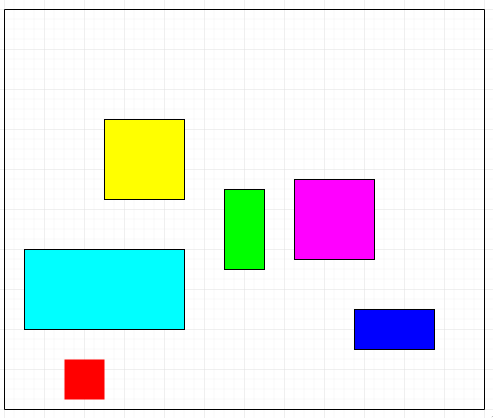
\includegraphics[width=6cm]{./pics/elements.png}
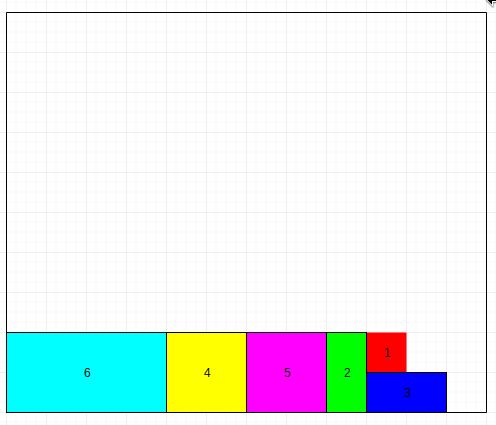
\includegraphics[width=6cm]{./pics/optimal.png}
\end{center}
\caption{Elementos en una colocación cualquiera y en una óptima}
\end{figure}

La generación de los individuos de la población inicial se realizará como se ha explicado anteriormente con números aleatorios, de tal modo que todos los bloques queden en el rectángulo definido por las esquinas (0,0) y (16, 15), por lo que el fitness mínimo de los individuos iniciales sería $(12*10)^{-1} = 120^{-1} = 0.008333...$. Para facilitar los cálculos y la representación, y dado que el tamaño más pequeño del lado de los bloques es 1 en x e y, se redondearán los valores a la unidad.

\begin{center}
\begin{tabular}{r|c c|c c|c c|c c|c c|c c}
Individuo & $x_1$ & $y_1$ & $x_2$ & $y_2$ & $x_3$ & $y_3$ & $x_4$ & $y_4$ & $x_5$ & $y_5$ & $x_6$ & $y_6$ \\ \hline
0 & 1 & 3 & 2 & 5 & 8  & 4 & 6  & 7 & 10 & 5 & 2 & 3 \\
1 & 7 & 1 & 7 & 5 & 10 & 8 & 7  & 1 & 3  & 6 & 4 & 7 \\
2 & 6 & 6 & 7 & 1 & 0  & 1 & 7  & 8 & 7  & 3 & 0 & 2 \\
3 & 3 & 6 & 1 & 7 & 1  & 9 & 10 & 0 & 4  & 7 & 6 & 4 \\
4 & 4 & 1 & 7 & 1 & 2  & 5 & 0  & 2 & 0  & 4 & 7 & 2 \\
5 & 5 & 5 & 9 & 3 & 2  & 5 & 5  & 6 & 8  & 7 & 5 & 3 \\
\end{tabular}
\end{center}

\begin{figure}[h]
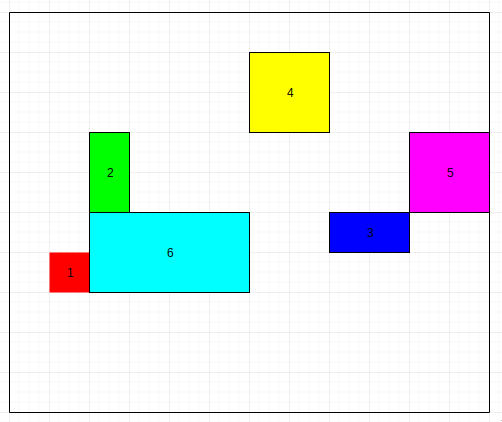
\includegraphics[width=5cm]{./pics/indiv1.png}
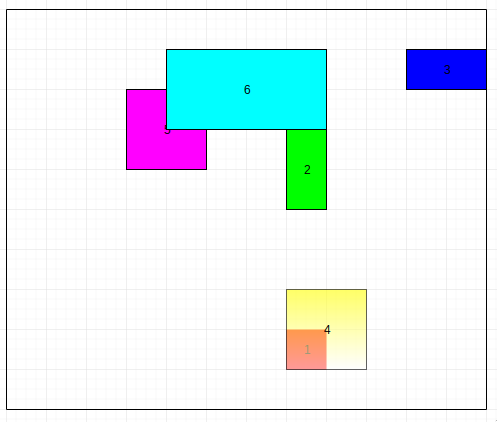
\includegraphics[width=5cm]{./pics/indiv2.png}
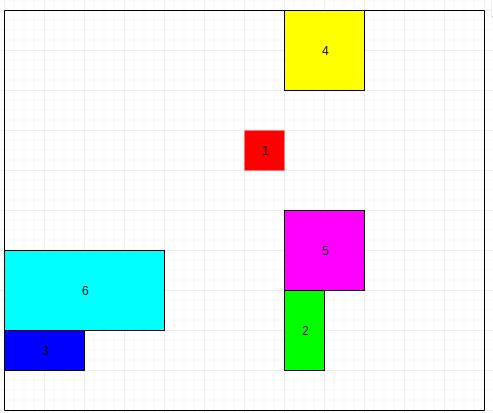
\includegraphics[width=5cm]{./pics/indiv3.png} \\
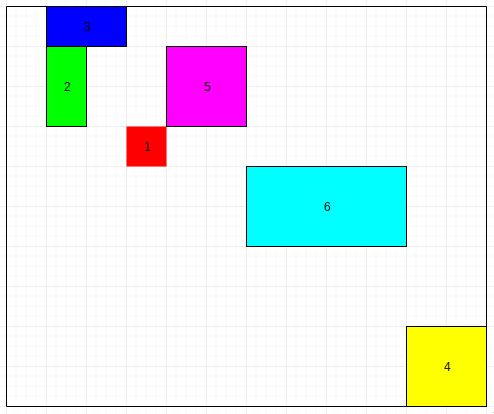
\includegraphics[width=5cm]{./pics/indiv4.png}
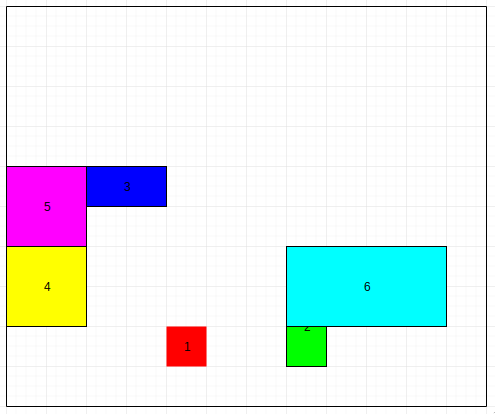
\includegraphics[width=5cm]{./pics/indiv5.png}
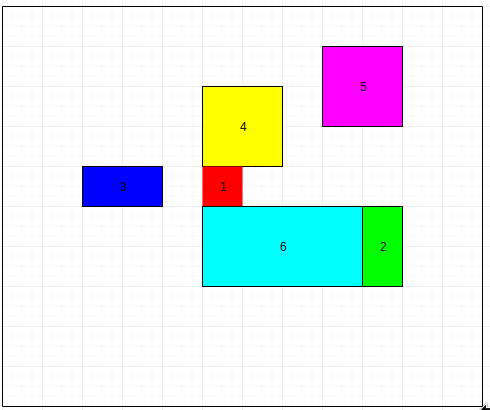
\includegraphics[width=5cm]{./pics/indiv6.png}
\caption{Representación gráfica de los 6 individuos}
\end{figure}
\subsection{Ciclo generacional}
\subsubsection{Cálculo del fitness}
Antes de calcular el fitness debemos resolver los solapamientos de los individuos 1 y 5, en los cuales los desplazamientos mínimos son los siguientes:
\begin{enumerate}
\item Individuo 1: mover bloque 4 a la derecha una unidad
\item Individuo 1: mover bloque 6 a la derecha una unidad
\item Individuo 5: mover bloque 6 a la derecha una unidad \footnote{Esto provoca una disminución del fitness, aún pudiendo existiendo otros desplazamientos que no modifiquen el fitness, o que lo mejoren. Se podría modificar la función fitness para que, en caso de solapamiento, buscara la mejor posición para el bloque solapado según el fitness. Esto agiliza la búsqueda de soluciones, pero es computacionalmente más costoso.}
\end{enumerate}
Una vez resueltos estos conflictos, podemos pasar al cálculo del fitness:
\begin{center}
\begin{tabular}{r|c|c|c|c|c|l|l}
Individuo & min $x$ & min $y$ & max $x$ & max $y$ & Área & Fitness & Ranking\\ \hline
0 & 1 & 3 & 12 & 9  & 66  & 0.0151515 & 3\\
1 & 3 & 1 & 12 & 9  & 72  & 0.0138889 & 4\\
2 & 0 & 1 & 9  & 10 & 81  & 0.0123457 & 5\\
3 & 1 & 0 & 12 & 10 & 110 & 0.0090909 & 6\\
4 & 0 & 1 & 11 & 6  & 55  & 0.0181818 & 2\\
5 & 2 & 3 & 10 & 9  & 48  & 0.0208333 & 1\\
\end{tabular}
\end{center}

\subsubsection{Selección}
La probabilidad de selección de cada individuo se muestra en la siguiente tabla:
\begin{center}
\begin{tabular}{r|l|l|l}
Individuo & $f_i$ & $p_i$ & Acumulado\\ \hline
0 & 0.0151515 &  0.169 & 0.169\\
1 & 0.0138889 &  0.155 & 0.324\\ 
2 & 0.0123457 &  0.138 & 0.462\\
3 & 0.0090909 &  0.102 & 0.564\\
4 & 0.0181818 &  0.203 & 0.767\\
5 & 0.0208333 &  0.233 & 1.000\\ \hline \hline
Total & 0.089492 & 1.000 \\
\end{tabular}
\end{center}
Si generamos números aleatorios entre 0 y 1 podemos seleccionar cuantos individuos necesitemos. Como ejemplo vamos a seleccionar 2 para mostrar el cruce y uno para mutación.

Con los siguientes números aleatorios (0.21, 0.53 y 0.74), seleccionamos para el cruce a los individuos 1 y 3 y al individuo 4 para la mutación.

\subsubsection{Cruce}
Realicemos un cruce de 2 puntos entre los individuos 1 y 3. Primero hemos de seleccionar los puntos de corte, por ejemplo entre los genes 3 y 5 (ambos incluidos)

\begin{center}
\begin{tabular}{r|c c|c c|c c|c c|c c|c c}
Individuo & $x_1$ & $y_1$ & $x_2$ & $y_2$ & $x_3$ & $y_3$ & $x_4$ & $y_4$ & $x_5$ & $y_5$ & $x_6$ & $y_6$ \\ \hline
1     & 7 & 1 & 7 & 5 & 10 & 8 & 7  & 1 & 3  & 6 & 4 & 7 \\
3     & 3 & 6 & 1 & 7 & 1  & 9 & 10 & 0 & 4  & 7 & 6 & 4 \\
nuevo & 7 & 1 & 7 & 5 & 1  & 9 & 10 & 0 & 4  & 7 & 4 & 7 \\
nuevo & 3 & 6 & 1 & 7 & 10 & 8 & 7  & 1 & 3  & 6 & 6 & 4 \\
\end{tabular}
\end{center}

\subsubsection{Mutación}
Aunque probablemente la mutación no hubiera sucedido aleatoriamente vamos a ``forzar'' una mutación para mostrar cómo se realizaría, en este caso mutación por intercambio recíproco. El individuo a mutar es el 2, si seleccionamos al azar 2 números entre el 1 y el 6 (puesto que el individuo sólo tiene un cromosoma con 6 genes) obtenemos la siguiente mutación (genes 3 y 4):

\begin{center}
\begin{tabular}{r|c c|c c|c c|c c|c c|c c}
Individuo & $x_1$ & $y_1$ & $x_2$ & $y_2$ & $x_3$ & $y_3$ & $x_4$ & $y_4$ & $x_5$ & $y_5$ & $x_6$ & $y_6$ \\ \hline
4     & 4 & 1 & 7 & 1 & 2  & 5 & 0  & 2 & 0  & 4 & 7 & 2 \\
nuevo & 4 & 1 & 7 & 1 & 0  & 2 & 2  & 5 & 0  & 4 & 7 & 2 \\
\end{tabular}
\end{center}


\subsubsection{Reemplazo}
Aunque el diseño del algoritmo especifica que se emplea un reemplazo por gap generacional de manera que se reemplaze $\frac{1}{3}$ los elementos, para mostrar la mutación y el cruce en el mismo paso, se reemplazan la mitad de los elementos. En el ejemplo que hemos desarrollado, cada gen generado sustituirá a uno de los genes desde el cual ha sido creado.

\subsubsection{Población resultante}
La población resultante se puede ver en la siguiente tabla e imágenes.

\begin{center}
\begin{tabular}{r|c c|c c|c c|c c|c c|c c}
Individuo & $x_1$ & $y_1$ & $x_2$ & $y_2$ & $x_3$ & $y_3$ & $x_4$ & $y_4$ & $x_5$ & $y_5$ & $x_6$ & $y_6$ \\ \hline
0 & 1 & 3 & 2 & 5 & 8  & 4 & 6  & 7 & 10 & 5 & 2 & 3 \\
1 & 7 & 1 & 7 & 5 & 1  & 9 & 10 & 0 & 4  & 7 & 4 & 7 \\
2 & 6 & 6 & 7 & 1 & 0  & 1 & 7  & 8 & 7  & 3 & 0 & 2 \\
3 & 3 & 6 & 1 & 7 & 10 & 8 & 7  & 1 & 3  & 6 & 6 & 4 \\
4 & 4 & 1 & 7 & 1 & 0  & 2 & 2  & 5 & 0  & 4 & 7 & 2 \\
5 & 5 & 5 & 9 & 3 & 2  & 5 & 5  & 6 & 8  & 7 & 5 & 3 \\
\end{tabular}
\end{center}

\begin{figure}[h]
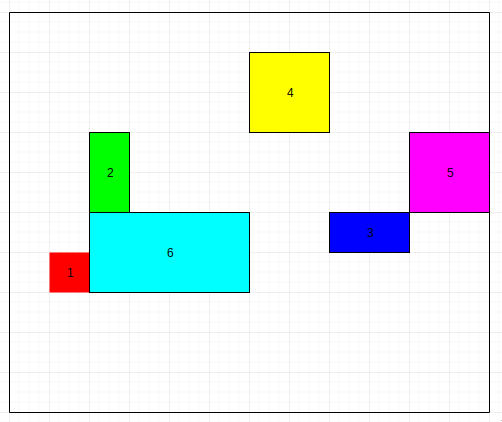
\includegraphics[width=5cm]{./pics/indiv1.png}
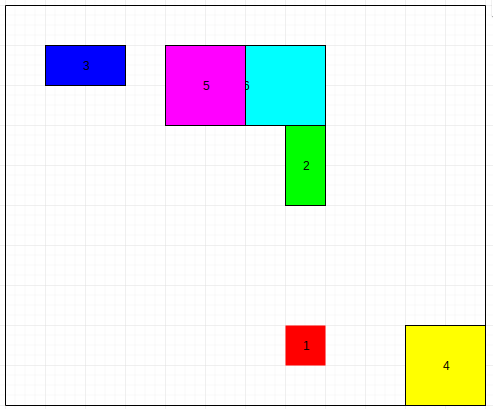
\includegraphics[width=5cm]{./pics/new1.png}
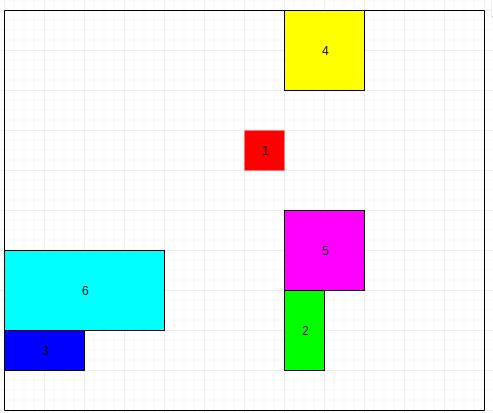
\includegraphics[width=5cm]{./pics/indiv3.png} \\
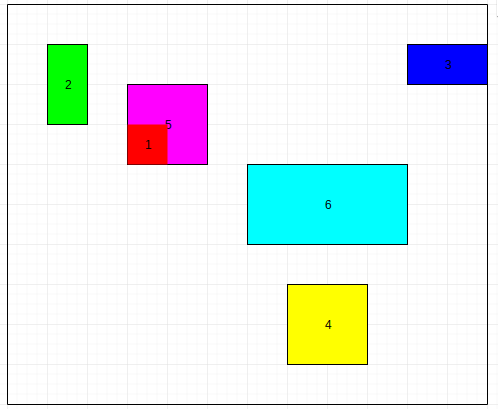
\includegraphics[width=5cm]{./pics/new3.png}
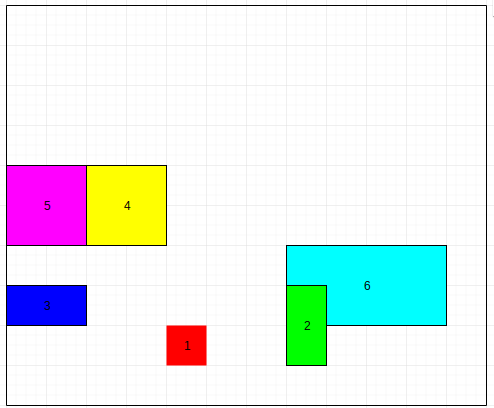
\includegraphics[width=5cm]{./pics/new4.png}
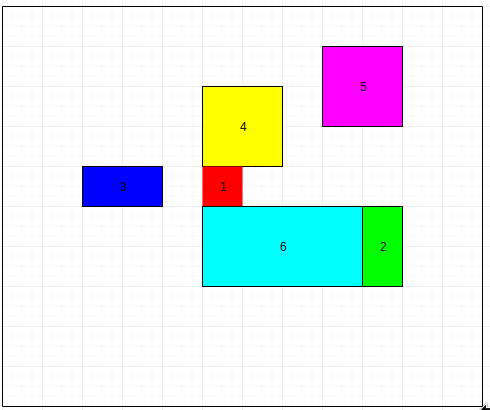
\includegraphics[width=5cm]{./pics/indiv6.png}
\caption{Representación gráfica de los 6 individuos después de la primera generación}
\end{figure}
\end{document}